\section{Network architecture and model training}
Our implementation of image ranking using neural networks closely follows the approach provided by \cite{wang2014learning} (refer Figure \ref{fig:architecture}). The deep ranking framework consists of 3 critical components as enlisted below:
 

\begin{itemize}
    \item \textbf{Triplet sampling layer} - Image triplets containing query image $(I_{i})$, positive example $(I_{i}^{+})$ and a negative example $(I_{i}^{-})$ are the inputs to the architecture. These are then fed into three identical deep neural networks. The deep neural network computes the embedding of an image as  $I_{i}:f(I_{i})$\in $R_{d}$ where f(.) is the deep neural network (i.e P/Q/R), 'd' is the dimension of the function embedding, 'R' represents the real number space.
    \item \textbf{Feature extraction} - \cite{wang2014learning} uses a novel multi-scale based neural network architecture as a feature extractor. The model produces feature embedding for images which are then fed into the ranking layer. In our implementation we use a modified version of Resnet-50 as the feature extractor, i.e, P, Q and R as shown in figure \ref{fig:architecture}, is a Resnet50 architecture as opposed to the multi-scale Convnet architecture proposed in \cite{wang2014learning}.
    \item \textbf{Ranking layer} - It computes the triplet margin loss on a single triplet as shown in \ref{eqn1}, which is then back propagated through the network. 
    
\end{itemize}

\subsection{Triplet sampling}
The triplet sampling layer supplies the model with triplets such that one pair is similar to each other and the other pair is dissimilar. We consider two images to be similar if they are from the same class and are dissimilar if they are from different classes. The procedure for sampling triplets is as follows:

\begin{enumerate}
    \item From the collection of all images, sample a subsequence $(I_{i})$ randomly (uniform random). 
    \item Let $(I_{i})$ belong to class $C_i$.
    \item Select another class $(I_{i}^{+})$ from the same class $C_i$ randomly (uniform random) such that $(I_{i}^{+}) != (I_{i})$.
    \item Randomly (uniform random) choose another class $C_j$ such that $C_j != C_i$ from the set of all classes $C$.
    \item Sample $(I_{i}^{-})$ from class $C_j$ randomly (uniform random).
\end{enumerate}

\subsection{Feature extraction}
The sampled triplets are required to be passed through a model which acts as a feature extractor whose output is then fed to the ranking layer. In this work, we choose Resnet-50 as the feature extractor after experimenting with numerous other DNN models (including Inception, Resnet-108, Resnet-18, VGG-16 etc). While some models like resnet-18, VGG-16 were not complex enough to extract relevant features from the data, the bigger complicated models like Inception, Resnet-108 etc consumed a lot of GPU run time. Hence Resnet-50 is a practical choice this work. We replace the last fully connected layer of Resnet 50 with a new fully connected layer of hidden size 2000.

\subsection{Loss function and model optimization}

The image ranking model is optimized based on the triplet margin loss, given by: 
\begin{equation}\label{eqn1}
\mathcal{L} =  min(D(f(I_{i}^{+}), f(I_{i})) - D(f(I_{i}^{-}), f(I_{i})) + M, 0)
\end{equation}

where $\mathcal{L}$ is the loss obtained for a triplet, D(.) is a distance function (we use the euclidean distance), f(.) is the neural network P(/Q/R, in this case, Resnet50), $(I_{i})$ is the query image, $(I_{i}^{-})$ is the negative example and $(I_{i}^{+})$ is the positive example and M is the margin (typically set to 1). The model is trained using the stochastic gradient descent algorithm with a batch size 40, a learning rate of 0.0001 with the Adam optimizer.

\subsubsection{Adaptive triplet margin loss}


% \begin{figure}[tp!]
% \centerline{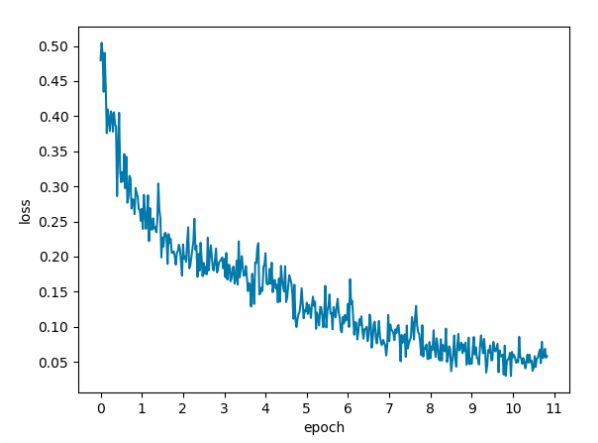
\includegraphics[scale=0.5]{imgs/Train_loss.png}}
%     \caption{Residual learning: building block}
%     \label{fig:loss}
% \end{figure}
